\chapter{Research on type annotations\label{related_work}}
% research on type annotations?
\section{Researching type annotations}

The most prevalent research method to investigate if existing type annotations in Python code are correct is to sample a dataset of source code and then run type checking against it \cite{di_grazia_evolution_2022, lin_towards_large_scale_2023, rak-amnouykit_taleoftwo_2020, xu_how_well_static_2023}. This creates data on type coverage and type errors. To get data on defect detection fixed defects are sampled. By adding correct type annotations to the defective source code before the fix, researchers can detect if a type checker could have detected the defect.

% Bug olis varmaan helpompi sana käyttää ja tutumpi lukijoille, mut käytän defectiä. Lähteet jakautui tän suhteen aika 50/50.

\section{Usage of type annotations}

Annotations often stay unchanged for an extended period after being added \cite{di_grazia_evolution_2022}. Projects can be categorized into three patterns: regular annotation, type sprints, and occasional usage. In a dataset of 9655 Python projects the used pattern correlated with the number of contributors, with regular annotation averaging the highest contributor count of 62, type sprints 45, and occasional use projects averaging 25 contributors. A motivation of type annotations helping coordination between higher numbers of active contributors was hypothesized to explain this phenomenon.

\begin{figure}
    \centering
    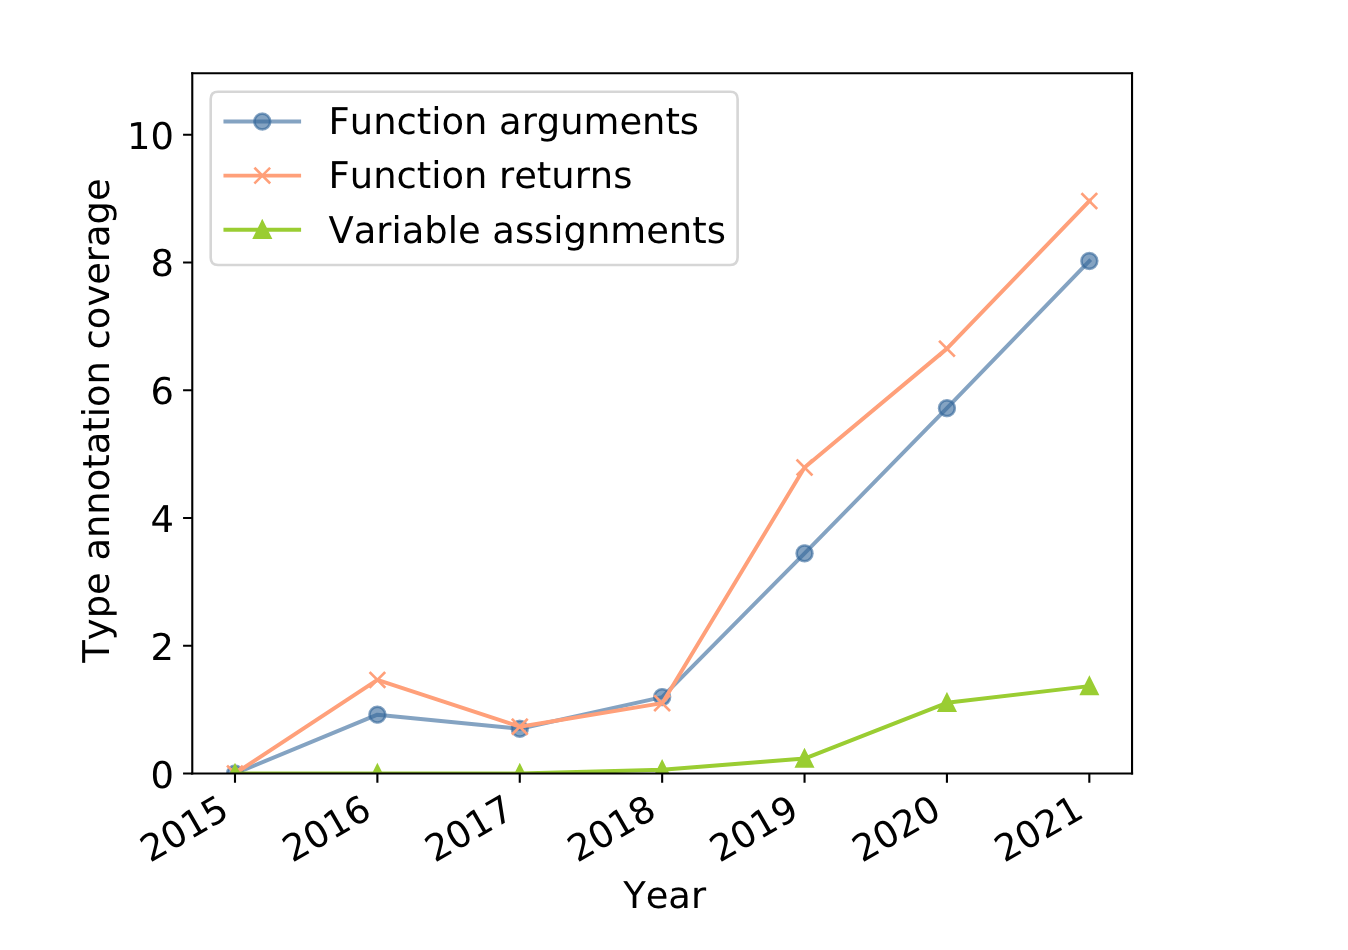
\includegraphics[width=0.5\linewidth]{Screenshot 2024-12-05 at 15.37.59.png}
    \caption{Python type annotation evolution from 2015 to 2021 \cite{di_grazia_evolution_2022}}
    \label{fig:annotation-evolution}
\end{figure}
From the introduction of Python type annotations in 2015 they reached around 8\% function argument and return coverage by 2021 in an analysis of 9655 Python projects \cite{di_grazia_evolution_2022}. 

Using a single large Python project picked for representativeness (TensorFlow) \cite{lin_towards_large_scale_2023}, the ratio of functions that have type annotations rose from 5\% in 2019 to 39\% in 2022. This increase seems consistent with the general rate in \ref{fig:annotation-evolution}.
% \pagebreak %secret TODO: this is here because otherwise a single line goes to the next page, ensure in final version this is necessary
The trend of adoption for type annotations has been increasing, but it should be noted that the proportion of typed code was not very high by 2022.

\subsection{Incorrect type annotations}

A 2020 study of Python type annotations usage patterns \cite{rak-amnouykit_taleoftwo_2020} found that even though type annotations and type checking are being adopted more widely, only 15\% of the 2678 codebases analysed successfully type checked with Mypy. A study of 9655 most popular Python projects on GitHub in 2022 found that 78\% of commits that had type annotations contained type errors \cite{di_grazia_evolution_2022}.

Some errors that Mypy and Pytype find are false positives \cite{rak-amnouykit_taleoftwo_2020}. False positives can be caused by differences in type checking setup to the one originally used by the project. Different type checkers, type checker versions, and configurations affect what type patterns are raised as errors, and which errors are detected.

\subsection{Empirical benefits}

Making use of types and type checking can allow development time detection of various program defects. In a retroactive analysis it was found that up to 11\% of a sample of patched defects could have been found at development time with types \cite{khan_empirical_2022}. Another analysis \cite{xu_how_well_static_2023} found that in a sample of 40 type-related defects 35\% could be detected without type annotations and 73\% with annotations.

Both experienced and inexperienced programmers make significant amounts of type-related mistakes when working with Python \cite{khan_empirical_2022}. These consist of: using variables before initialising them, null safety errors, and re-using variables with values of different types. This implies that both experienced and inexperienced programmers can derive benefits from types, since type checking helps fix these mistakes.

Pydantic is a widely adopted data validation library for Python that enables runtime data validation using type annotations \cite{pydanticdev_welcome_nodate}. There is no academic research available on its effectiveness or popularity. Common use cases include web services where incoming data has to be validated anyway, type annotations enabling a simple way to write schemas for the data.